\section{Experiments, source audits, and what the measurements establish}
\label{sec:experiments}

\subsection{Reproducible input and measurement protocol}

The native input is the pinned 106-case marked-parallelity corpus.  Its
SHA-256 digest is recorded in \code{PROVENANCE.json} and in every native
audit.  The export reconstructs each source from the triangulation and
normal coordinates, reconstructs it a second time through the independent
reference implementation, and checks exact agreement before extracting
any matrix.  No precomputed geometric matrix is accepted merely because
its filename says that it came from the source.

The timing experiment imports three separate namespaces: the exact pinned
baseline, the source-reuse-only ablation, and the final speed patch.  It runs
five rounds for every case, randomizing the order of the three variants
within each case and round with recorded seed 20261012.  Each observation
includes the native whole-cut producer and, on a complete result, the
independent whole-cut certificate checker.  The program compares the
entire returned objects, including statistics, censuses, and certificates,
on every repetition.  All comparisons pass.  There are 92 complete and
14 inconclusive outcomes in each timing variant.

The environment is CPython 3.12.14 on Linux x86-64, with
\code{perf_counter_ns} as the timer.  The raw observations, Python version,
platform string, source hashes, and aggregation rule accompany the article.
They are measurements on this host, not hardware-independent constants.
Two subsequently corrected docstrings differ from the measured snapshot;
their recorded hashes reproduce exactly and the executable abstract syntax
trees are unchanged.  The delivery provenance records both versions.

\subsection{Full-query speed and a controlled ablation}

\begin{table}[htbp]
\centering
\begin{tabular}{lrrr}
\toprule
Variant & Production (s) & Independent replay (s) & Full query (s)\\
\midrule
Pinned baseline & 32.2088 & 23.4109 & 55.7582\\
Source reuse only & 32.1755 & 22.4004 & 54.8330\\
Final speed patch & 27.3450 & 15.1712 & 42.6671\\
\midrule
Baseline/final ratio & $1.1779$ & $1.5431$ & $1.3068$\\
\bottomrule
\end{tabular}
\caption{Sum, over all 106 cases, of the five-round median for each
measured quantity.  The median of a sum need not equal the sum of medians,
so the production and replay columns need not add exactly to the full-query
column.  No lower-forest portfolio is included in these timings.}
\label{tab:paired-times}
\end{table}

The aggregate full-query reduction is
$1-42.667140636/55.758189326=23.48\%$.  The median, over cases, of the
within-case paired baseline/final ratio is $1.3004$.  These two summaries
agree closely here, although they answer different questions: one weights
large cases by their wall time, while the other describes a typical case.
Source reuse alone changes aggregate full-query time by a factor of only
$1.0169$.  The larger final gain is consistent with the profile's finding
that orbit contraction and transport dominate this particular workload.
It would be incorrect to attribute the entire improvement to caching
source geometry.

\begin{figure}[htbp]
\centering
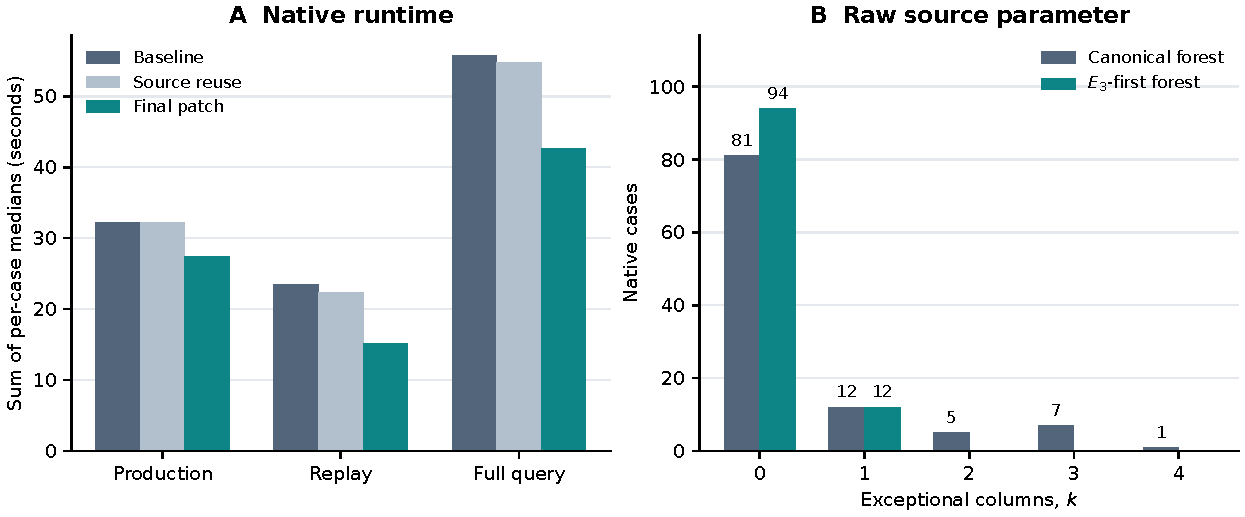
\includegraphics[width=\textwidth]{figures/native_results.pdf}
\caption{Two distinct native results.  Left: complete-query timing of
the behavior-preserving speed patch.  Right: distribution of the raw
exceptional-column count before and after the proved lower-forest parameter
optimization.  The right panel is a source audit, not a timing experiment.}
\label{fig:native-results}
\end{figure}

A separate synthetic experiment isolates endpoint mapping and verifies
exact equality with the preceding naive formula.  It uses equal numbers
of pairings and static gaps, from 64 through 4096, with five paired rounds.
At 4096 pairings the median naive mapper time is 2.3172 seconds and the
median prefix mapper time is 0.004870 seconds.  Their ratio is approximately
476; the median of the five paired ratios is approximately 509.  These
are deliberately labelled mapper-only numbers.  They are not the speedup
of the native recognizer or even of its entire orbit checker.

\begin{figure}[htbp]
\centering
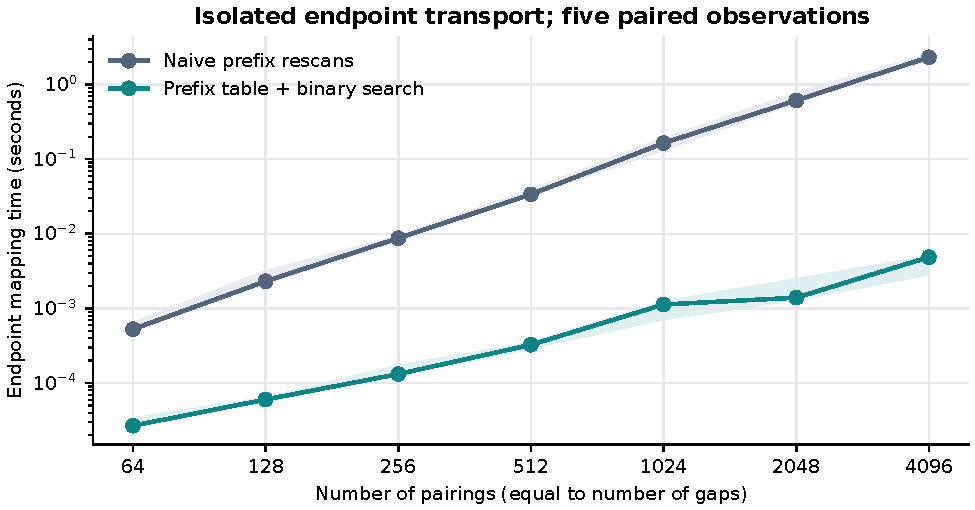
\includegraphics[width=0.83\textwidth]{figures/prefix_scaling.pdf}
\caption{Synthetic endpoint-remapping measurements, with medians and
the range of the five observations.  Both axes are logarithmic.  The theorem
establishes the asymptotic improvement; this experiment isolates the
implementation that realizes it.  Source authentication and other orbit
operations are outside this plot.}
\label{fig:prefix-scaling}
\end{figure}

\subsection{Fresh native parameters and exact finite-core outcomes}

The native exporter checks the raw unsigned occurrence bound on every
one-handle column: total at most three, and at most two for a corner handle.
It also exports the canonical lower forest and a forest attaining
\(\kappa=|E_3|-r_G(E_3)\).  The resulting distributions are:

\begin{center}
\begin{tabular}{lrrrrr}
\toprule
Lower-forest policy & $k=0$ & $k=1$ & $k=2$ & $k=3$ & $k=4$\\
\midrule
Canonical & 81 & 12 & 5 & 7 & 1\\
$E_3$ first & 94 & 12 & 0 & 0 & 0\\
\bottomrule
\end{tabular}
\end{center}

For the canonical matrices, 89 cases have no nonfree special SCC, seven
have one, eight have two, one has three, and one has four.  Their ideal
counts are respectively 1, 2, 4, 8, and 16.  In this raw corpus the surviving
special-SCC orders happen to be antichains, so the ideal refinement does
not further reduce the Boolean state count.  It is a proved structural
improvement whose benefit requires a different order structure.  After
$E_3$-first optimization, the nonfree dimensions are zero in 94 cases,
one in ten, and two in two; the largest ideal count is four.

\begin{table}[htbp]
\centering
\begin{tabular}{lrr}
\toprule
Finite supplied-matrix result & Canonical lower forest & $E_3$ first\\
\midrule
Old two-row solver: success & 81 & 94\\
Old two-row solver: unsupported/inconclusive & 25 & 12\\
Exact history solver: success & 100 & 106\\
Exact history solver: finite infeasibility & 6 & 0\\
Deterministic width solver: success & 100 & 106\\
Randomized ideal solver: success & 100 & 106\\
\bottomrule
\end{tabular}
\caption{The native \emph{raw core} finite problems.  The six unsuccessful
canonical cases yield exact finite negatives in deterministic search and
inconclusive outputs in randomized discovery.  Every positive certificate
passes the separate finite verifier.  These counts are not whole-cut
handlebody counts.}
\label{tab:finite-core}
\end{table}

All 212 finite instances---106 with each lower-forest policy---were also
checked by an independent exhaustive spanning-tree and literal-peeling
oracle.  It enumerated 136 spanning trees for each policy and agreed with
the exact solvers on every instance.  The native dual rank is at most one
in this corpus.  Thus this experiment authenticates a useful native domain
and detects real lower-forest effects, but does not empirically stress the
new theorem at large dual rank.  In particular, all 106 optimized positives
are already found by the deterministic mandatory-group candidate followed
by peeling; none needs a nonzero determinant discovery.  The algebraic
implementation is exercised separately against explicit basis expansions.

The six raw-core rescues are the pilot Fibonacci cases with indices
04, 06, 08 and 10, together with \code{pilot/lst_4_9/0} and
\code{pilot/finite_trefoil/0}.
All 100 prior raw-core successes are preserved by the optimized forest on
this corpus.  That empirical preservation is not asserted as a theorem
for arbitrary inputs.

\subsection{Five additional whole-cut certificates}

A separate, optional producer portfolio first tries the maintained
planner and then two bounded lower-forest policies: $E_3$ first and reverse
edge order.  The finite core proof is replayed, and any completed whole-cut
packet is submitted to the unchanged public whole-cut verifier.  The adapter
uses a private producer-module instance; it does not replace a public
module's planner or alter the certificate schema.

\begin{center}
\begin{tabular}{P{0.57\textwidth}P{0.31\textwidth}}
\toprule
New full-certificate case & Successful alternative\\
\midrule
\code{pilot/fibonacci_lst_04/0} & $E_3$ first\\
\code{pilot/fibonacci_lst_06/0} & $E_3$ first\\
\code{pilot/lst_4_9/0} & $E_3$ first\\
\code{pilot/finite_trefoil/0} & $E_3$ first\\
\code{pachner23_5_8_2/mixed} & Reverse order\\
\bottomrule
\end{tabular}
\end{center}

Each new packet contains the original source, coordinates, and complete
native certificate, with its hash recorded in the audit.  Combining these
five verified positives with the maintained 92 gives 97 complete whole-cut
censuses out of 106.  The original speed patch continues to produce exactly
the original 92 outputs; the coverage increase belongs to the separately
dispatched research portfolio.

The larger Fibonacci cases with indices eight and ten now pass raw core
cancellation but stop at annular attachment.  The finite figure-eight
positive target still stalls in the whole-cut core path in the bounded
search.  These observations identify a geometric continuation problem,
not a reason to relax unsigned cancellation or certificate checks.

A historical Regina oracle audit, tied to this same corpus hash, identifies
eight genuine all-handlebody misses among the original fourteen refusals;
the other six contain at least one non-handlebody piece.  This classification
is explicitly labelled historical in the package; it was not recomputed
as part of the timing run.  The three saved interface obstructions in the
preceding forest report belong to the latter category.  Seeking geometric
moves that preserve the whole cut yet turn all of their components into
handlebodies would therefore be a misguided positive target.  If sphere
capping is intended, it needs its own changed terminal specification and
certificate.

\subsection{Independent finite identities and hostile inputs}

The new unit suite has 15 test methods.  Its exhaustive family covers all
4096 combinations of a binary $3\times2$ matrix and three edge records
chosen from two loops, one eligible edge, and an unavailable edge.  It also
checks 320 weighted instances with wider exceptional columns, 180 small
posets including chains and antichains, all 256 three-variable Boolean
truth tables, resource limits, and certificate/source mutations.

The independent mathematical audit programs add the following checks:

\begin{itemize}
\item 800 matrices, 2836 tree/matrix pairs, and 46\,127 exceptional
  schedules checked against literal peeling;
\item 700 covering instances and 1377 determinant evaluations compared
  with direct common-basis polynomial expansion;
\item 650 Boolean-sieve matrices, 2300 tree/matrix pairs, 8657 activation
  table entries, and 711 determinant-versus-basis comparisons;
\item 1800 random posets on one through nine elements, containing 47\,467
  enumerated ideals, with direct zeta, inverse, maximal-element and filter
  identities checked;
\item 650 further weighted instances, with up to five rows in an
  exceptional support, checked directly against the delivered width and
  randomized implementations and an independent tree/peeling oracle.
\end{itemize}

The focused maintained-runtime regression passes 100 tests, and the separate
portfolio suite passes nine, for 109 distinct implementation tests in total.
These are additional to the 15 finite-solver test methods.  The runtime suite includes
the independent gap arithmetic and source-mutation checks described in
\cref{sec:implementation-prefix}.  Test identities, seeds, commands and raw
reports are included so that a reader can distinguish proof, finite testing,
and a native source-authenticated result.  Finite audits do not replace the
proofs, and passing selected runtime tests does not claim that every test
elsewhere in the large repository was rerun.
